\chapter{Introduction}

Modelling and replicating the effects of acoustic systems has been of continued interest to a number of industries, from the creation of scale models for concert halls to the generation of individualised audio in video games~\cite{Rindel2000}. Acoustic modelling is not only a tool for those wishing to design acoustic systems, but may be of increasing interest for those wishing to experience an acoustic system\footnote{In this context we consider an acoustic system as whole i.e. sound sources, receivers, the propagation medium and the domain boundaries} from the comfort of the home or office~\cite{Tsingos2009}. Simulating the acoustic behaviour of large systems with multiple sources and receivers may not be a trivial undertaking, with significant computational resources required to model such systems. 

\section{Problem Definition}
\begin{wrapfigure}{r}{0.35\textwidth}
  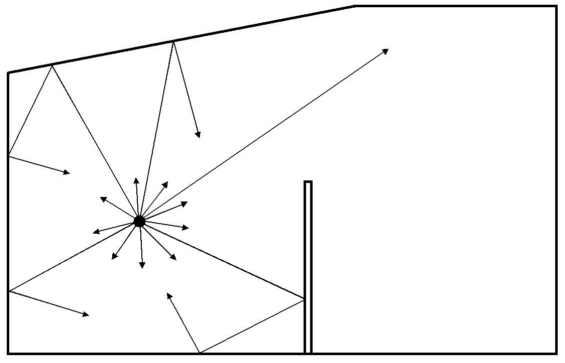
\includegraphics[width=0.34\textwidth]{./graphics/raytracing.png}
  \caption{2D Representation of Ray Tracing Concept~\cite{Elorza2005}}
\end{wrapfigure}

Current commercially available acoustic modelling tools for large (cathedrals, arenas, video game maps etc) electroacoustic simulations rely on assumptions based around plane wave propagation. These models are only accurate when assuming that detail of the domain features are significantly larger than the wavelengths of interested, and that no diffraction effects occur~\cite{Schmalle2011}. These ray based methods such as the image source method and ray or beam tracing methods approximate the performance of the system and simulation domain without solving the full wave physics of an acoustic system~\cite{Monks1996a}. These methods have been successfully used to approximate large systems at mid and high frequencies, but may not accurately simulate low frequency wave propagation and wave interaction.\\

Wave based acoustic modelling methods such as the Finite Element Method (FEM) and Boundary Element Method (BEM) have been are currently implemented in commercial software packages, and are often used to model complex acoustic systems such as loudspeakers and other transducers. However, these packages are difficult to apply to simulating large domain problems, due to the computational resource limitations that are inherent with numerical solutions to wave based methods. Modelling large 3D domains even at lower frequencies can have extreme memory requirements, and may also require significant computation time to 'crunch the numbers' and solve for adequate amounts of time. One commercial FEM package known as Comsol has recently added ray tracing to the acoustics tools, potentially to accommodate this restriction~\cite{Jensen2016}.\\

\section{Aim of the Study}

The aim of this study is to test three numerical methods of solving the acoustic wave equation that result in time domain solutions. These methods will be implemented in the Matlab $\textregistered $ language tested for speed of time step execution with consecutively large domains. The methods of interested in this studying are the finite difference time domain method (FDTD), the sparse finite difference time domain method (SFDTD) and the pseudospectral time domain method (PSTD). The outcome of this study will be the identification of a method that may warrant further optimisation for large domains and could be potentially used for accurately modelling large electroacoustic systems and venues. To summaries, these are the objectives in this project:\\

\begin{itemize}
\item Explore and implement FDTD method in 1D, 2D and 3D
\item Explore and implement PSTD method in 1D, 2D and 3D
\item Implement PSTD method partially absorbing boundaries
\item Explore and implement SFDTD method in 1D, 2D and if possible 3D
\item Validate these models propagate sound appropriately
\item Benchmark the execution speed for these methods in different size models
\item Write a report detailing the study
\end{itemize}

\section{Format of the Report}
At first the acoustic wave equation will be derived, and some properties of large room acoustics will be discussed. Following this the finite difference time domain, sparse finite difference time domain and pseudo spectral time domain methods for solving the acoustic wave equation will be introduced, including equation derivation and Matlab code examples. Following this the software validation will be discussed, and finally the time step execution times will be evaluated including profiling to determine the slowest part of code execution.\\

